\documentclass[conference]{IEEEtran}
\IEEEoverridecommandlockouts
\usepackage{cite}
\usepackage{amsmath,amssymb,amsfonts}
\usepackage{algorithmic}
\usepackage{graphicx}
\usepackage{textcomp}
\usepackage{xcolor}
\usepackage{url}
\usepackage{tikz}
\usetikzlibrary{arrows.meta,positioning,shapes.geometric,shapes.misc}
% Shared TikZ styles for ClimateFact architecture diagrams
\tikzset{
  process/.style={
    rectangle, rounded corners=3pt, draw, thick, fill=black!5,
    minimum width=2.8cm, minimum height=0.7cm,
    text centered, font=\footnotesize, text width=2.6cm
  },
  datastore/.style={
    cylinder, draw, thick, shape border rotate=90, aspect=0.15,
    fill=black!10, minimum width=2.2cm, minimum height=0.8cm,
    text centered, font=\tiny, text width=2.0cm
  },
  io/.style={
    trapezium, trapezium left angle=75, trapezium right angle=105,
    draw, thick, fill=white, minimum width=2.0cm, minimum height=0.6cm,
    text centered, font=\footnotesize
  },
  subgraph/.style={
    rectangle, rounded corners=5pt, draw=black!60, dashed, thick,
    fill=black!3, inner sep=6pt
  },
  arrow/.style={-Stealth, thick, black!80},
  annot/.style={font=\scriptsize\itshape, text=black!60},
}

\def\BibTeX{{\rm B\kern-.05em{\sc i\kern-.025em b}\kern-.08em
    T\kern-.1667em\lower.7ex\hbox{E}\kern-.125emX}}
\begin{document}

\title{ClimateFact: A RAG workflow for climate change fact verification\\
\thanks{This work was developed at the School of Computer Science and Informatics, University of Costa Rica.}
}

\author{
\IEEEauthorblockN{1\textsuperscript{st} Ariel Ar\'{e}valo Alvarado}
\IEEEauthorblockA{\textit{School of Computer Science and Informatics} \\
\textit{University of Costa Rica}\\
San Jos\'{e}, Costa Rica \\
ariel.arevalo@ucr.ac.cr}
\and
\IEEEauthorblockN{2\textsuperscript{nd} Andrik Acu\~{n}a Castillo}
\IEEEauthorblockA{\textit{School of Computer Science and Informatics} \\
\textit{University of Costa Rica}\\
San Jos\'{e}, Costa Rica \\
andrik.acuna@ucr.ac.cr}
\and
\IEEEauthorblockN{3\textsuperscript{rd} Anthony S\'{a}nchez Ram\'{i}rez}
\IEEEauthorblockA{\textit{School of Computer Science and Informatics} \\
\textit{University of Costa Rica}\\
San Jos\'{e}, Costa Rica \\
anthony.sanchezramirez@ucr.ac.cr}
\and
\IEEEauthorblockN{4\textsuperscript{th} Erick Andr\'{e}s Sibaja Li}
\IEEEauthorblockA{\textit{School of Computer Science and Informatics} \\
\textit{University of Costa Rica}\\
San Jos\'{e}, Costa Rica \\
erick.sibaja@ucr.ac.cr}
}

\IEEEaftertitletext{\begin{center}\itshape June 4, 2025\end{center}}
\maketitle

\begin{abstract}
This project presents a fact-checking workflow called ClimateFact that aims to evaluate climate change-related statements using trustworthy scientific knowledge bases. Motivated by the prevalence of climate misinformation and the lack of accessible, domain-specific verification tools, ClimateFact uses Retrieval-Augmented Generation (RAG) to identify and explain inconsistencies between claims and authoritative sources such as the IPCC reports.

The workflow generates a knowledge base using embeddings and regex-based indexing informed by domain-specific ontologies. It then retrieves relevant passages using a multi-step retrieval and re-ranking pipeline, followed by a natural language inference (NLI) model to assess the factual alignment of claims.

Finally, an LLM generates grounded explanations marking contradictions with references. The methodology includes reproducible evaluation pipelines to measure retrieval accuracy, factual consistency, and explanation quality.
\end{abstract}

\begin{IEEEkeywords}
fact-checking, climate change, RAG, NLI, retrieval-augmented generation
\end{IEEEkeywords}

\section{Introduction}
Climate change is one of the most pressing challenges facing humanity today. Its growing impact on ecosystems, the global economy, and people's daily lives makes this phenomenon a priority for governments, scientists, and citizens alike. According to the IPCC report, the human influence on the climate system is undeniable and is directly linked to historical greenhouse gas emissions \cite{ipcc2022}. However, despite this scientific consensus, climate change continues to be the subject of misinformation, with erroneous claims that distort public perception and hinder the implementation of effective policies.

In this context, various international figures such as Ant\'{o}nio Guterres, Secretary-General of the United Nations, have made urgent calls to action, highlighting the need to take drastic measures to prevent even more severe consequences \cite{planelles2022}. Furthermore, experts such as Fern\'{a}ndez Muerza (2022) have emphasized that effective communication about climate change is essential for citizens to understand the magnitude of the problem and make informed, responsible decisions \cite{fernandez2022}. However, when information sources are unreliable or contain incorrect claims, the risk of making misguided decisions increases significantly. Therefore, it is crucial to have tools that help filter and verify available information. This raises the question: Is it possible to build an AI agent that detects inconsistencies in climate change claims using retrieval-augmented generation techniques?

The general objective of this work is to build a computational tool capable of identifying and describing inconsistencies in climate change-related claims through automatic fact-checking techniques. This proposal falls within contemporary fact-checking approaches applied to scientific and environmental topics.

To achieve this purpose, the following specific objectives are proposed:

\begin{enumerate}
    \item Build a reliable knowledge base on climate change from official documents issued by recognized institutions, such as the IPCC.

    \item Design an automated workflow that retrieves relevant evidence from the knowledge base to contrast it against external claims.

    \item Develop a mechanism for generating and evaluating inconsistencies that details the differences between claims and retrieved evidence, as well as a validation process to measure its effectiveness.
\end{enumerate}

To this end, a methodology based on Retrieval-Augmented Generation (RAG) will be employed, combining generative models with semantic retrieval techniques. This approach will allow contrasting claims against authoritative technical content, providing precise and efficient validation.

The development of this system not only seeks to contribute to semantic verification in the context of climate change but also to strengthen initiatives against environmental misinformation through the use of artificial intelligence. By providing a reliable mechanism for validating climate change claims, this intelligent agent can facilitate more informed decision-making in both academic settings and public policy formulation. Additionally, it could be a useful tool for governments, non-governmental organizations, and companies dealing with climate change, improving the quality and effectiveness of responses to this global challenge.

The second section of the paper presents related work, reviewing previous research related to automatic claim verification and the use of language models in the context of climate change. Then, the conceptual framework is presented, detailing the theoretical and technical foundations supporting the proposal. The methodology section describes the system design and development, from knowledge base construction to RAG model application. Subsequently, the results obtained from the system implementation are presented, and finally, a discussion is included analyzing the findings, model limitations, and potential future applications.

\section{Estado del arte}

En años recientes, la inteligencia artificial se ha consolidado como un área clave en el desarrollo tecnológico, dando lugar a un incremento significativo en las investigaciones vinculadas a sus múltiples aplicaciones. Este auge se explica por la capacidad de la IA para ofrecer respuestas innovadoras y eficaces a problemas complejos en distintos sectores, entre ellos la educación, el entorno empresarial, la salud y el medio ambiente. Bajo esta perspectiva, el presente estado del arte explora los principales avances científicos en el uso de la inteligencia artificial para tareas como el procesamiento del lenguaje natural, la verificación automática de datos y la creación de modelos lingüísticos de gran escala.

Primero tenemos el trabajo realizado por Chavarría Muñoz~\cite{chavarria2022}, quien desarrolló un prototipo de aplicación web para la detección de noticias falsas en español, integrando algoritmos de clasificación como \textit{Support Vector Machine}, \textit{Random Forest} y \textit{Passive Aggressive Classifier}, junto con técnicas de procesamiento de lenguaje natural como análisis de sentimiento, modelado de temas y detección de lenguaje soez. El estudio utilizó un corpus balanceado de 1248 noticias (mitad falsas y mitad verdaderas), alcanzando niveles de precisión cercanos al 72\% con el clasificador \textit{Random Forest}. A través del uso de herramientas como Python, Streamlit y Heroku, el prototipo permitió que los usuarios ingresaran el título y cuerpo de una noticia, recibiendo como resultado un porcentaje estimado de veracidad junto con métricas lingüísticas asociadas, lo que representa un aporte relevante en la automatización del análisis crítico de contenido digital en español~\cite{chavarria2022}.

Luego tenemos el trabajo de Rey Morales~\cite{rey2025fakenews}, quien desarrolló un modelo para la detección de noticias falsas combinando diversas técnicas de procesamiento de lenguaje natural y algoritmos de clasificación. En su estudio se implementaron enfoques como TF-IDF, Bag of Words, Word2Vec y el modelo transformer DistilBERT, junto con clasificadores como regresión logística, Support Vector Machines y Random Forest. Además, aplicó técnicas como reducción de dimensionalidad con PCA y validación cruzada para mejorar la precisión. Una de las principales conclusiones fue que, si bien los modelos avanzados como BERT lograron altos niveles de precisión (superiores al 99\%), el análisis contextual de elementos externos a la noticia ---como comentarios, fuente y similitud con otras noticias--- es esencial para alcanzar predicciones más fiables. Este trabajo contribuye al estado del arte al ofrecer una comparación exhaustiva de métodos y evidenciar la importancia del contexto en la detección automatizada de desinformación.

Por ultimo tenemos el trabajo desarrollado por Mafla Checa~\cite{mafla2021noticias}, titulado \textit{``Identificación automática de noticias falsas en español utilizando técnicas de minería de datos y procesamiento de lenguaje natural''}. Este estudio lo que propone es una metodología completa que abarca desde la construcción de un corpus de noticias ecuatorianas hasta la implementación y comparación de modelos de clasificación supervisada. El autor recopila manualmente un conjunto de noticias reales y falsas provenientes de medios nacionales y páginas de política, y posteriormente aplica técnicas de \textit{procesamiento de lenguaje natural (PLN)} como la lematización, remoción de \textit{stop words} y representación vectorial mediante \textit{TF-IDF}. Para abordar el desequilibrio en las clases, se emplea la técnica de sobremuestreo \textit{SMOTE}. El estudio evalúa el desempeño de diferentes modelos de clasificación, incluyendo \textit{Support Vector Machines (SVM)}, \textit{Naive Bayes}, \textit{Random Forest} y \textit{Boosting}, utilizando métricas como la precisión, \textit{F1-score} y curvas \textit{ROC}. Los resultados mostraron que los modelos más eficientes fueron SVM y Boosting, con un rendimiento considerablemente superior cuando se aplicó un preprocesamiento exhaustivo de los textos.

\section{Marco conceptual}

En esta sección se explican los conceptos clave que se utilizan a lo largo del proyecto. La intención es brindar al lector una base de comprensión sobre los términos técnicos y teóricos, de forma que pueda seguir el desarrollo del trabajo con mayor facilidad.

\subsection{Procesamiento de Lenguaje Natural (PLN)}
El Procesamiento de Lenguaje Natural (PLN) se refiere a la capacidad de las computadoras para interpretar, comprender y utilizar lenguajes humanos de forma efectiva. Esta área facilita tanto la creación de programas orientados a la manipulación y análisis de texto, como el diseño de modelos que simulan los procesos cognitivos del ser humano relacionados con el lenguaje~\cite{cortez2021pln}.

\subsection{Embeddings Semánticos}

Según Mikolov et al.~\cite{mikolov2013distributed}, los \textit{word embeddings} son representaciones vectoriales de palabras en un espacio continuo de múltiples dimensiones, donde cada dimensión refleja características o conceptos latentes compartidos por distintos términos. Esta forma de organización no se corresponde necesariamente con categorías semánticas explícitas definidas por los seres humanos, sino que responde a patrones internos aprendidos por el modelo. Por ejemplo, aunque palabras como ``rey'' y ``reina'' no sean sinónimos ni pertenezcan a una misma categoría gramatical, sus vectores resultan cercanos en el espacio de embeddings, reflejando una relación semántica implícita entre ambas.

\subsection{Modelos Transformer}
Los modelos Transformer constituyen una arquitectura de aprendizaje profundo diseñada para procesar secuencias de manera paralela, sin recurrir a estructuras recurrentes. Se basan en un mecanismo de atención que permite a cada elemento de la entrada ponderar la importancia de los demás elementos del conjunto, lo que facilita el aprendizaje de relaciones a largo plazo. Entre sus características más destacadas se encuentra el uso de la autoatención multicabeza, que mejora la capacidad del modelo para capturar patrones complejos desde múltiples perspectivas. Gracias a su eficiencia computacional y rendimiento sobresaliente, esta arquitectura se ha convertido en la base de los modelos de lenguaje más avanzados en la actualidad~\cite{garcia2021transformers}.

\subsection{Inferencia Textual Natural (NLI)}
La Inferencia Textual Natural (NLI, por sus siglas en inglés) es una tarea fundamental del Procesamiento de Lenguaje Natural que consiste en evaluar la relación lógica entre una premisa y una hipótesis. El objetivo es determinar si la hipótesis puede considerarse verdadera (\textit{entailment}), falsa (\textit{contradiction}), o indeterminada (\textit{neutral}) a partir del contenido de la premisa. Esta tarea también se conoce como Reconocimiento de la Implicación Textual (\textit{Recognizing Textual Entailment, RTE}) y suele utilizarse como prueba de referencia para evaluar el grado de comprensión del lenguaje de los modelos de PLN~\cite{bowman2015nli}.


\subsection{Recuperación Aumentada por Generación (RAG)}
La arquitectura RAG, por sus siglas en inglés (\textit{Retrieval-Augmented Generation}), se presenta como una solución eficaz para enriquecer las capacidades de los modelos de lenguaje de gran escala (LLM) sin necesidad de reentrenamiento. Su funcionamiento se basa en dos componentes principales: la indexación semántica de documentos mediante representaciones vectoriales, y el uso de la información recuperada como contexto adicional para que el modelo de lenguaje genere respuestas más precisas y confiables. Esta integración permite reducir la incidencia de errores o alucinaciones típicas de los LLM y adaptar sus respuestas a dominios específicos sin modificar sus parámetros base~\cite{sanchez2024rag}.


\subsection{Corpus Científico y Verificación de Afirmaciones}
La verificación automática de hechos requiere fuentes confiables. El corpus empleado corresponde al \textbf{informe de síntesis del Sexto Informe del IPCC} \cite{ipcc2022}, que proporciona información técnica validada sobre el cambio climático. Utilizar un corpus con estructura científica garantiza coherencia y confiabilidad en las inferencias.

\subsection{Pipeline en PLN}
Un pipeline de PLN es una secuencia estructurada de tareas de procesamiento lingüístico. En este trabajo, el pipeline incluye:

\begin{enumerate}
    \item Extracción y segmentación del corpus.
    \item Resolución de correferencias.
    \item Vectorización semántica.
    \item Recuperación contextual.
    \item Inferencia textual.
\end{enumerate}

Cada componente del pipeline está diseñado para preservar la coherencia semántica y facilitar la verificación lógica de afirmaciones externas.

\section{Methodology}

This work implements an automatic verification system for climate change claims, combining advanced natural language processing (NLP) techniques with a retrieval-augmented generation (RAG) approach. The complete pipeline is organized as a workflow composed of two stages: the construction of an embedding-based knowledge base from a scientific reference corpus, and assisted semantic inference to verify external claims through textual reasoning.

\subsection{Embedding-Based Knowledge-Assisted Semantic Verification Pipeline}


\subsubsection{Corpus extraction and preprocessing}
The Synthesis Report of the Sixth Assessment Report of the IPCC~\cite{ipcc2023}, in PDF format, was used as the knowledge source. To preserve the original semantic structure, the \texttt{MinerU} parser was applied, which transforms documents into Markdown with structural tags. In this way, images and footers were discarded to obtain a cleaner corpus.


\subsubsection{Coreference resolution and text segmentation}
Once the content was extracted, it was segmented at the paragraph level and processed with the \textbf{AllenNLP Coreference Model}, based on \textbf{SpanBERT-large}, to replace pronouns with their explicit antecedents. This step improves the referential coherence of the text and facilitates the comparison of all sentences with their explicit subjects. Then, sentence-level segmentation was applied, and regular expressions were used to correct separation errors introduced during the coreference resolution stage.

\subsubsection{Semantic vectorization of the corpus}
Each sentence was transformed into a 1,536-dimensional embedding using OpenAI's \textbf{text-embedding-3-small} model. These embeddings constitute a semantic knowledge base that encapsulates precise, contextualized scientific information from the IPCC, organized for efficient searches by semantic proximity.

\subsubsection{Hybrid concept index construction (regex + NER)}
In addition to purely semantic search, a concept index was built combining lexical rules and entity recognition. This is executed in three stages: (a) extraction by regular expressions defined on climate ontologies, (b) entity detection with \textit{spaCy} and NLTK, and (c) fusion and deduplication of results with priority given to confidence and text coverage.

\subsubsection{Hybrid retrieval and deduplication}
At query time, the external claim is analyzed with the same hybrid extractor; the resulting concepts are used as a filter on the index to obtain a relevant subset of sentences. Subsequently, semantic search by embedding similarity is performed within that subset. This combination produces more complete and relevant results.

\subsubsection{Contextual retrieval by embedding similarity}
The input claim is converted into an embedding using the same OpenAI model. Then, the cosine similarity between that embedding and all embeddings in the knowledge base is calculated. The most similar sentence is selected as contextual evidence for logical analysis.

The sets retrieved through hybrid search and independent semantic search are merged and subjected to a deduplication process to avoid redundant evidence.

\subsubsection{Logical inference via NLI}
Finally, the logical relationship between the reformulated claim and the retrieved evidence is evaluated using the \textbf{DeBERTa-Large-MNLI} model, specialized in natural language inference (NLI) tasks. The model classifies the relationship into one of the following categories:

\begin{itemize}
\item \textbf{Entailment}: The evidence implies the claim.
\item \textbf{Contradiction}: The claim conflicts with the evidence.
\item \textbf{Neutral}: The evidence neither confirms nor refutes the claim.
\end{itemize}

This approach allows verifying claims with explicit support from the IPCC scientific corpus, combining the robustness of semantic embeddings with the textual logical reasoning of state-of-the-art NLI models.

\subsection{Runtime application architecture}
Corpus preprocessing and hybrid index construction are executed \emph{outside} the inference graph, through standalone command-line scripts. In contrast, the verification application exposed to the end user is an interface that orchestrates a graph. This graph includes four subtasks: (i) claim segmentation, (ii) hybrid retrieval, (iii) contradiction detection via NLI, and (iv) generation of the explanatory response shown to the user.

The separation between resource construction and the inference graph facilitates incremental knowledge updates without interrupting the service, and allows deploying the application in lightweight environments where only online verification needs to be executed.

\subsection{Resource acquisition and management}

All resources are openly accessible:

\begin{itemize}
\item \textbf{Models}:
      \begin{itemize}
      \item \texttt{text-embedding-3-small} and \texttt{gpt-4o-mini}: OpenAI API with educational credits.
      \item \texttt{DeBERTa-Large-MNLI}: Docker image published in \textit{Microsoft}'s public container registry.
      \end{itemize}
\item \textbf{Data}: IPCC reports downloaded from the official repository (\url{https://www.ipcc.ch}).
\item \textbf{Tools}: \texttt{spaCy}, \texttt{NLTK}, \texttt{AllenNLP}, \texttt{LangGraph}, and \texttt{Streamlit}, all with permissive licenses.
\item \textbf{Compute}: one \texttt{Standard\_NC4as\_T4\_v3} node (\$0.53 USD/h) on AzureML for NLI inference.
\end{itemize}

These resources are obtained without prohibitive cost and meet open-access ethical requirements, facilitating the reproducibility of the study.

\section{Evaluación}

La evaluación del sistema ClimateFact se estructura en torno a una metodología reproducible que permite medir la efectividad de cada componente del flujo de verificación. El proceso evaluativo se fundamenta en la construcción de un conjunto de referencia (\textit{gold set}) y la aplicación de métricas estándar para sistemas de recuperación de información y clasificación textual.

\subsection{Construcción del conjunto de referencia}

Se construyó un conjunto de referencia compuesto por 400 pares de afirmación-evidencia extraídos del corpus científico del IPCC. Cada entrada del conjunto incluye una afirmación sobre cambio climático y el identificador del pasaje que constituye la evidencia más relevante dentro de la base de conocimiento. La selección de estos pares se realizó mediante un proceso semi-automático que garantiza la correspondencia semántica entre afirmaciones y evidencia.

Adicionalmente, se incorporaron casos de control que representan aproximadamente el 10\% del conjunto total. Estos casos incluyen: (i) afirmaciones sin evidencia correspondiente en el corpus, (ii) afirmaciones acompañadas de pasajes distractores que no proporcionan evidencia relevante, y (iii) afirmaciones deliberadamente ambiguas que permiten evaluar la robustez del sistema ante consultas imprecisas.

Para la evaluación específica del componente de inferencia lógica, cada par afirmación-evidencia fue etiquetado manualmente según la relación lógica que establece el pasaje respecto a la afirmación: \textit{entailment} (la evidencia implica la afirmación), \textit{contradiction} (la evidencia contradice la afirmación), o \textit{neutral} (la evidencia no permite confirmar ni refutar la afirmación).

\subsection{Métricas de evaluación de recuperación}

La calidad del subsistema de recuperación se evalúa mediante métricas estándar de sistemas de recuperación de información, aplicadas para diferentes valores de $k$ (número de documentos recuperados):

\begin{itemize}
\item \textbf{Recall@k}: Fracción de evidencia relevante recuperada entre los primeros $k$ resultados.
\item \textbf{Precision@k}: Fracción de documentos relevantes entre los $k$ documentos recuperados.
\item \textbf{MRR@k}: Reciprocal rank medio, que mide la posición del primer documento relevante en el ranking.
\item \textbf{nDCG@k}: Ganancia acumulativa descontada normalizada, que pondera la relevancia según la posición en el ranking.
\end{itemize}

Estas métricas se calculan de forma independiente para cada estrategia de recuperación (híbrida conceptual, semántica por embeddings, y combinación fusionada) con valores de $k \in \{1, 3, 5, 10\}$, permitiendo evaluar tanto la precisión como la exhaustividad del proceso de recuperación.

\subsection{Métricas de evaluación de inferencia lógica}

La efectividad del modelo de inferencia textual natural se evalúa mediante métricas de clasificación multiclase:

\begin{itemize}
\item \textbf{Exactitud global}: Fracción de predicciones correctas sobre el total de casos evaluados.
\item \textbf{Precisión, Recall y F1-score por clase}: Calculadas independientemente para cada etiqueta de relación lógica.
\item \textbf{Promedios macro y micro}: Agregación de métricas individuales para obtener una evaluación global del clasificador.
\item \textbf{Matriz de confusión}: Análisis detallado de errores de clasificación entre categorías.
\end{itemize}

\subsection{Protocolo de evaluación}

El protocolo de evaluación garantiza la reproducibilidad mediante la separación estricta entre datos de entrenamiento y evaluación. El conjunto de referencia se mantiene independiente de cualquier proceso de ajuste o calibración del sistema, asegurando una evaluación objetiva.

La evaluación se ejecuta de forma automatizada mediante scripts que procesan el conjunto completo de casos de prueba, registran las predicciones del sistema, y calculan todas las métricas especificadas. Los resultados se almacenan en formato estructurado que facilita tanto el análisis estadístico como la generación de reportes detallados.

Este enfoque metodológico permite identificar fortalezas y debilidades específicas en cada componente del sistema, proporcionando información valiosa para iteraciones futuras del desarrollo.

\section{Resultados}

La evaluación experimental del sistema ClimateFact se realizó sobre un conjunto de referencia de 400 casos de prueba, aplicando la metodología descrita en la sección anterior. Los resultados obtenidos se presentan organizados según los dos componentes principales del sistema: recuperación de evidencia e inferencia lógica textual.

\subsection{Rendimiento del subsistema de recuperación}

La evaluación del pipeline completo de recuperación, que integra búsqueda híbrida conceptual, recuperación semántica por embeddings y fusión de resultados, demuestra un rendimiento progresivamente mejorado conforme aumenta el número de documentos considerados. La Tabla~\ref{tab:retrieval_results} presenta los resultados obtenidos para diferentes valores de k.

\begin{table}[htbp]
\centering
\caption{Métricas de rendimiento del subsistema de recuperación}
\label{tab:retrieval_results}
\begin{tabular}{|c|c|c|c|c|c|}
\hline
\textbf{k} & \textbf{Recall} & \textbf{Precision} & \textbf{F1-Score} & \textbf{MRR} & \textbf{nDCG} \\
\hline
1 & 0.655 & 0.655 & 0.655 & 0.655 & 0.655 \\
\hline
3 & 0.865 & 0.355 & 0.483 & 0.751 & 0.845 \\
\hline
5 & 0.910 & 0.262 & 0.370 & 0.761 & 0.866 \\
\hline
10 & 0.938 & 0.184 & 0.252 & 0.765 & 0.876 \\
\hline
\end{tabular}
\end{table}

Para \textit{k=1}, el sistema alcanza un recall de 0.655, indicando que en aproximadamente dos tercios de los casos el documento más relevante se encuentra en la primera posición del ranking. La precisión coincide con el recall (0.655) dado que solo se considera un documento, resultando en un F1-score equivalente.

Al expandir la búsqueda a \textit{k=3}, el recall se incrementa significativamente a 0.865, lo que demuestra que el 86.5\% de la evidencia relevante se recupera dentro de los tres primeros resultados. Sin embargo, la precisión desciende a 0.355 debido a la inclusión de documentos menos relevantes, resultando en un F1-score de 0.483.

La tendencia se mantiene para \textit{k=5} y \textit{k=10}, con recalls de 0.91 y 0.9375 respectivamente, mientras que la precisión continúa disminuyendo (0.262 para \textit{k=5} y 0.184 para \textit{k=10}). Esta relación inversa entre recall y precisión es característica de sistemas de recuperación que priorizan la exhaustividad sobre la especificidad.

Las métricas de ranking muestran resultados consistentes: el MRR@k se estabiliza alrededor de 0.76 para valores superiores a \textit{k=3}, indicando que el primer documento relevante típicamente se encuentra en las primeras tres posiciones. El nDCG@k progresa de 0.655 (\textit{k=1}) a 0.876 (\textit{k=10}), reflejando la capacidad del sistema para posicionar documentos relevantes en posiciones altas del ranking.

\subsection{Rendimiento del modelo de inferencia lógica}

La evaluación del componente NLI reveló un rendimiento diferenciado según la clase de relación lógica analizada. El modelo alcanzó una exactitud global de 0.615 sobre 400 predicciones, con variaciones significativas entre categorías. La Tabla~\ref{tab:nli_results} presenta las métricas detalladas por clase, mientras que la Tabla~\ref{tab:confusion_matrix} muestra la matriz de confusión correspondiente.

\begin{table}[htbp]
\centering
\caption{Métricas de rendimiento del modelo NLI por clase}
\label{tab:nli_results}
\begin{tabular}{|l|c|c|c|}
\hline
\textbf{Clase} & \textbf{Precision} & \textbf{Recall} & \textbf{F1-Score} \\
\hline
ENTAILMENT & 0.524 & 0.675 & 0.590 \\
\hline
CONTRADICTION & 0.991 & 0.958 & 0.975 \\
\hline
NEUTRAL & 0.295 & 0.192 & 0.232 \\
\hline
\end{tabular}
\end{table}

\begin{table}[htbp]
\centering
\caption{Matriz de confusión del modelo NLI}
\label{tab:confusion_matrix}
\begin{tabular}{|l|c|c|c|}
\hline
\textbf{Verdadero \textbackslash Predicho} & \textbf{ENT} & \textbf{CON} & \textbf{NEU} \\
\hline
ENTAILMENT & 108 & 1 & 51 \\
\hline
CONTRADICTION & 1 & 115 & 4 \\
\hline
NEUTRAL & 97 & 0 & 23 \\
\hline
\end{tabular}
\end{table}

El análisis por clases evidencia disparidades notables en el rendimiento:

\textbf{Clase CONTRADICTION}: Exhibe el mejor rendimiento con una precisión de 0.991, recall de 0.958 y F1-score de 0.975. De 120 casos verdaderos de contradicción, el modelo identificó correctamente 115, con solo 1 falso positivo y 4 falsos negativos.

\textbf{Clase ENTAILMENT}: Muestra rendimiento intermedio con precisión de 0.524, recall de 0.675 y F1-score de 0.590. De 160 casos verdaderos de implicación, se identificaron correctamente 108, aunque el modelo generó 51 falsos negativos clasificados erróneamente como neutrales.

\textbf{Clase NEUTRAL}: Presenta el rendimiento más deficiente con precisión de 0.295, recall de 0.192 y F1-score de 0.232. De 120 casos neutrales, solo 23 fueron clasificados correctamente, mientras que 97 se clasificaron incorrectamente como implicación.

Los promedios macro resultantes son: precisión 0.604, recall 0.608 y F1-score 0.599, indicando un rendimiento moderado del clasificador con sesgo evidente hacia la detección de contradicciones.

\subsection{Análisis de la matriz de confusión}

La matriz de confusión revela patrones específicos de error en el modelo NLI. La confusión más frecuente ocurre entre las clases NEUTRAL y ENTAILMENT, donde 97 de 120 casos neutrales fueron clasificados erróneamente como implicación. Esta tendencia sugiere que el modelo tiende a interpretar relaciones neutras como evidencia de apoyo cuando existe solapamiento temático entre afirmación y evidencia.

En contraste, la clase CONTRADICTION muestra excelente separabilidad, con confusión mínima respecto a las otras categorías (1 falso positivo y 4 falsos negativos), lo que indica que el modelo es particularmente efectivo para identificar inconsistencias directas entre afirmaciones y evidencia.

\subsection{Cobertura del conjunto de referencia}

El análisis del conjunto de datos revela que 726 de las 846 entradas totales (85.8\%) contienen etiquetas de inferencia lógica, con una distribución equilibrada entre las tres categorías: 241 casos de implicación, 241 de contradicción y 244 neutrales. Esta distribución balanceada en el conjunto completo contrasta con el subconjunto evaluado, donde se observa una ligera predominancia de casos de implicación (160) sobre contradicción (120) y neutralidad (120).

Los resultados obtenidos establecen una línea base sólida para el sistema ClimateFact, identificando fortalezas en la recuperación de evidencia y la detección de contradicciones, así como áreas de mejora específicas en la clasificación de relaciones neutrales.

\section{Discusión}

Los resultados experimentales revelan características específicas del sistema ClimateFact que requieren análisis contextualizado respecto a su aplicación práctica en la detección de contradicciones climáticas.

\subsection{Interpretación de métricas de recuperación}

El comportamiento observado en las métricas de recuperación refleja trade-offs inherentes en sistemas de verificación de hechos. La disminución progresiva de la precisión conforme aumenta $k$ (de 0.655 para $k{=}1$ a 0.184 para $k{=}10$) representa una dilución esperada de la relevancia, donde cada incremento en el número de documentos recuperados introduce resultados menos pertinentes al conjunto final.

Sin embargo, desde la perspectiva de la detección de contradicciones, el recall constituye la métrica de mayor importancia práctica. Para invalidar una afirmación climática, basta con identificar \textit{al menos una} contradicción fundamentada en evidencia científica autorizada. Bajo esta premisa, el recall de 0.91 para $k{=}5$ resulta altamente satisfactorio, sugiriendo que el sistema recupera exitosamente evidencia contradictoria en más del 90\% de los casos evaluados.

La configuración de $k{=}5$ representa un equilibrio eficiente entre exhaustividad de recuperación y carga computacional para el componente NLI posterior. Esta parametrización minimiza el número de inferencias lógicas requeridas mientras mantiene capacidades de recuperación prácticamente óptimas.

\subsection{Evaluación del ranking híbrido}

El MRR estabilizado en 0.76 para valores de $k \geq 3$ evidencia la efectividad del pipeline híbrido propuesto. Considerando que la estrategia combina recuperación conceptual por regex, extracción de entidades nombradas, y búsqueda semántica mediante embeddings \texttt{text-embedding-3-small} de OpenAI, este rendimiento sugiere una sinergia positiva entre los métodos de recuperación complementarios.

La ausencia de reranking explícito más allá del ordenamiento por similitud semántica limita la interpretabilidad directa de las métricas nDCG obtenidas. No obstante, la progresión consistente del nDCG@k (de 0.655 a 0.876) indica que el sistema posiciona efectivamente documentos relevantes en posiciones superiores del ranking, validando la arquitectura híbrida implementada.

\subsection{Rendimiento especializado en detección de contradicciones}

El desempeño excepcional del modelo NLI en la clase CONTRADICTION (F1-score de 0.975) resulta particularmente relevante dado el objetivo específico del sistema. Esta especialización coincide con los requerimientos funcionales de ClimateFact, donde la detección precisa de inconsistencias constituye el caso de uso primario.

La distribución asimétrica de errores, concentrada principalmente en la confusión NEUTRAL-ENTAILMENT, sugiere un sesgo del modelo hacia la identificación de relaciones de apoyo en presencia de solapamiento temático. Este comportamiento, aunque problemático para aplicaciones de clasificación general, no compromete significativamente la funcionalidad central del sistema de detección de contradicciones.

La supremacía en la detección de contradicciones podría atribuirse tanto a características intrínsecas del modelo DeBERTa-Large-MNLI como a patrones distribucionales presentes en sus datos de entrenamiento. Investigaciones futuras podrían explorar si esta especialización refleja un sesgo arquitectural del modelo o una característica emergente de los corpus utilizados durante su entrenamiento.

\subsection{Implicaciones para sistemas de verificación climática}

Los resultados demuestran la viabilidad técnica de sistemas automatizados para la detección de desinformación climática. La combinación de alta recuperación de evidencia relevante y detección precisa de contradicciones establece fundamentos sólidos para herramientas de verificación de hechos especializadas en el dominio climático.

Las limitaciones identificadas, particularmente en la clasificación de relaciones neutrales, representan oportunidades de mejora que no comprometen la utilidad práctica inmediata del sistema. Futuras iteraciones podrían beneficiarse de estrategias de reranking más sofisticadas y ajustes específicos para mejorar la discriminación entre clases neutrales y de implicación.

\section{Conclusión}

Este trabajo presentó ClimateFact, un flujo basado en RAG para la verificación automatizada de afirmaciones sobre cambio climático contra fuentes científicas autorizadas. El sistema integra recuperación híbrida, inferencia de lenguaje natural y generación de explicaciones fundamentadas en un pipeline reproducible.

La evaluación experimental demostró un sólido desempeño en la recuperación, con un recall de 0.91 para $k=5$, lo que indica que la evidencia relevante se recupera exitosamente en más del 90\% de los casos evaluados. El componente NLI alcanzó un F1-score de 0.975 para la clase CONTRADICTION, confirmando la efectividad del sistema en su tarea principal de detección de inconsistencias factuales.

Sin embargo, el sistema exhibe una debilidad notable en la clasificación de la clase NEUTRAL, donde 97 de 120 casos neutrales fueron clasificados erróneamente como ENTAILMENT. Esta limitación, aunque no es crítica para la detección de contradicciones, reduce la confiabilidad del sistema como clasificador de alineación factual de propósito general.

El trabajo futuro debe abordar la confusión NEUTRAL--ENTAILMENT mediante ajuste fino con datos NLI específicos del dominio, explorar estrategias de reranking más sofisticadas para mejorar la precisión de la recuperación, e investigar la integración de verificación multilingüe de afirmaciones para ampliar la aplicabilidad del sistema más allá de fuentes en idioma inglés.


\bibliographystyle{IEEEtran}
\bibliography{references}

\appendix
\section{Diagramas de Arquitectura}
\label{sec:appendix-diagrams}

\begin{figure*}[t]
\centering
\resizebox{0.45\textwidth}{!}{% Diagram 1: Runtime Inference Pipeline
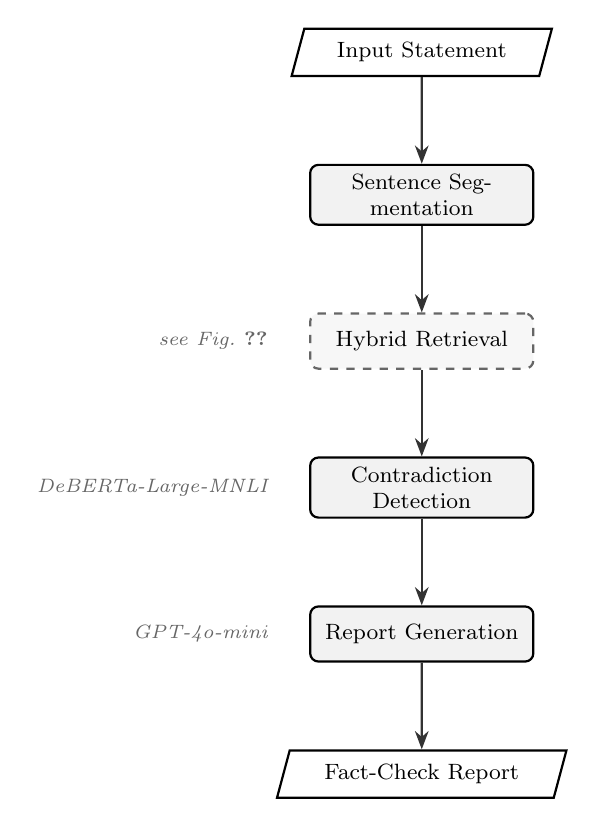
\begin{tikzpicture}[node distance=1.1cm]
  % Nodes
  \node[io] (input) {Input Statement};
  \node[process, below=of input] (seg) {Sentence Segmentation};
  \node[process, below=of seg, draw=black!60, dashed, fill=black!3] (ret)
    {Hybrid Retrieval};
  \node[process, below=of ret] (nli) {Contradiction Detection};
  \node[process, below=of nli] (gen) {Report Generation};
  \node[io, below=of gen] (output) {Fact-Check Report};

  % Arrows
  \draw[arrow] (input) -- (seg);
  \draw[arrow] (seg) -- (ret);
  \draw[arrow] (ret) -- (nli);
  \draw[arrow] (nli) -- (gen);
  \draw[arrow] (gen) -- (output);

  % Annotations
  \node[annot, left=0.4cm of ret] {see Fig.~\ref{fig:retrieval}};
  \node[annot, left=0.4cm of nli] {DeBERTa-Large-MNLI};
  \node[annot, left=0.4cm of gen] {GPT-4o-mini};
\end{tikzpicture}
}
\caption{Pipeline de inferencia en tiempo de ejecución. Cada afirmación de entrada fluye a través de cuatro etapas: segmentación, recuperación híbrida, detección de contradicciones vía NLI y generación del reporte.}
\label{fig:pipeline}
\end{figure*}

\begin{figure*}[t]
\centering
\resizebox{0.85\textwidth}{!}{% Diagram 3: Knowledge Base Construction Pipeline
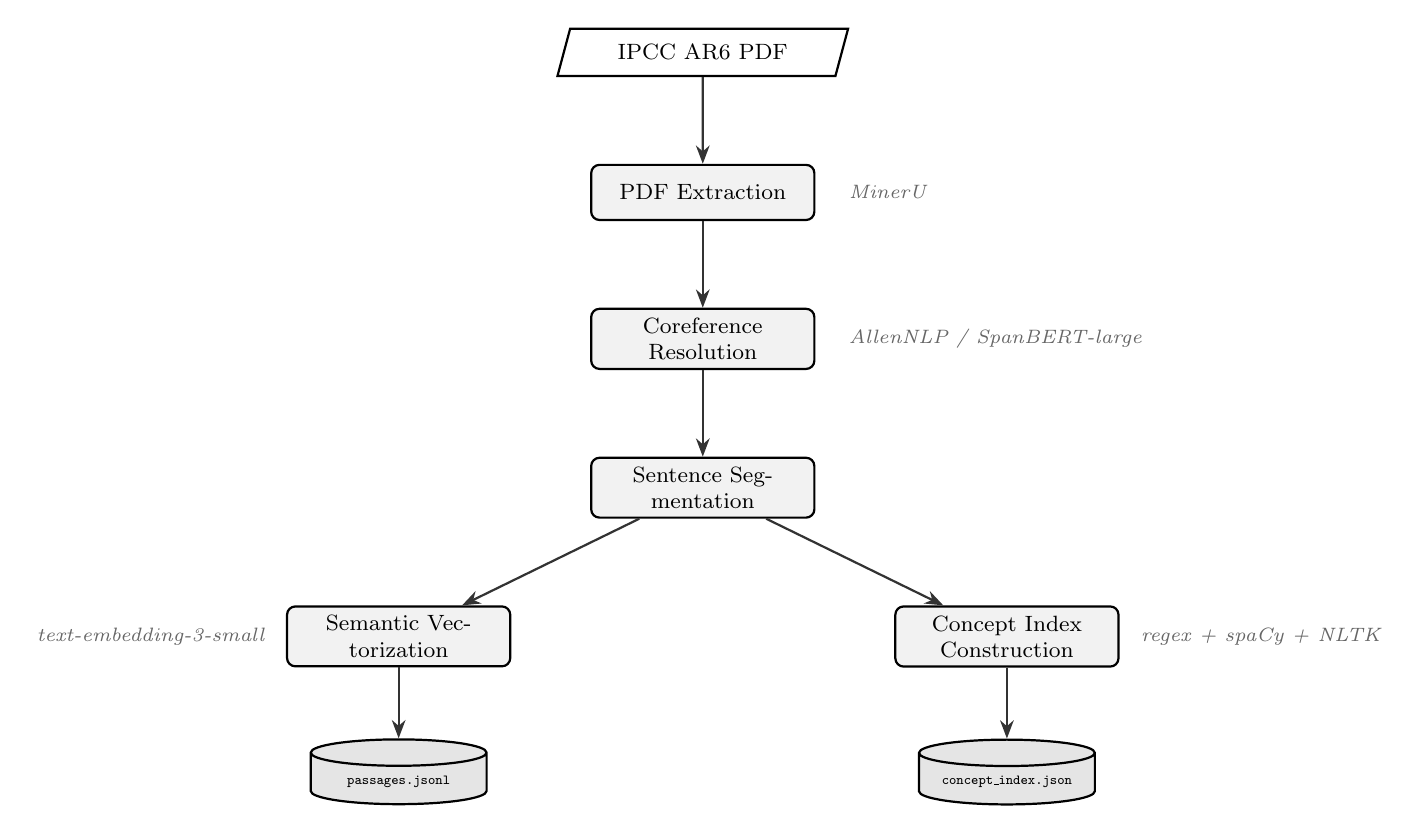
\begin{tikzpicture}[node distance=1.1cm]
  % Linear chain
  \node[io] (pdf) {IPCC AR6 PDF};
  \node[process, below=of pdf] (extract) {PDF Extraction};
  \node[process, below=of extract] (coref) {Coreference Resolution};
  \node[process, below=of coref] (sent) {Sentence Segmentation};

  % Fork into two branches
  \node[process, below left=1.1cm and 1.0cm of sent] (vec)
    {Semantic Vectorization};
  \node[process, below right=1.1cm and 1.0cm of sent] (cidx)
    {Concept Index Construction};

  % Data stores — larger for readability
  \node[datastore, below=0.9cm of vec] (passages)
    {\texttt{passages.jsonl}};
  \node[datastore, below=0.9cm of cidx] (index)
    {\texttt{concept\_index.json}};

  % Arrows — linear chain
  \draw[arrow] (pdf) -- (extract);
  \draw[arrow] (extract) -- (coref);
  \draw[arrow] (coref) -- (sent);

  % Fork arrows
  \draw[arrow] (sent) -- (vec);
  \draw[arrow] (sent) -- (cidx);

  % To data stores
  \draw[arrow] (vec) -- (passages);
  \draw[arrow] (cidx) -- (index);

  % Annotations
  \node[annot, right=0.3cm of extract] {MinerU};
  \node[annot, right=0.3cm of coref] {AllenNLP / SpanBERT-large};
  \node[annot, left=0.15cm of vec, anchor=east] {text-embedding-3-small};
  \node[annot, right=0.15cm of cidx, anchor=west] {regex + spaCy + NLTK};
\end{tikzpicture}
}
\caption{Pipeline de construcción offline de la base de conocimiento. El documento fuente del IPCC se procesa en dos artefactos: un almacén de pasajes vectorizados y un índice híbrido de conceptos.}
\label{fig:kb-construction}
\end{figure*}

\begin{figure*}[t]
\centering
\resizebox{0.95\textwidth}{!}{% Diagram 2: Hybrid Retrieval Subgraph
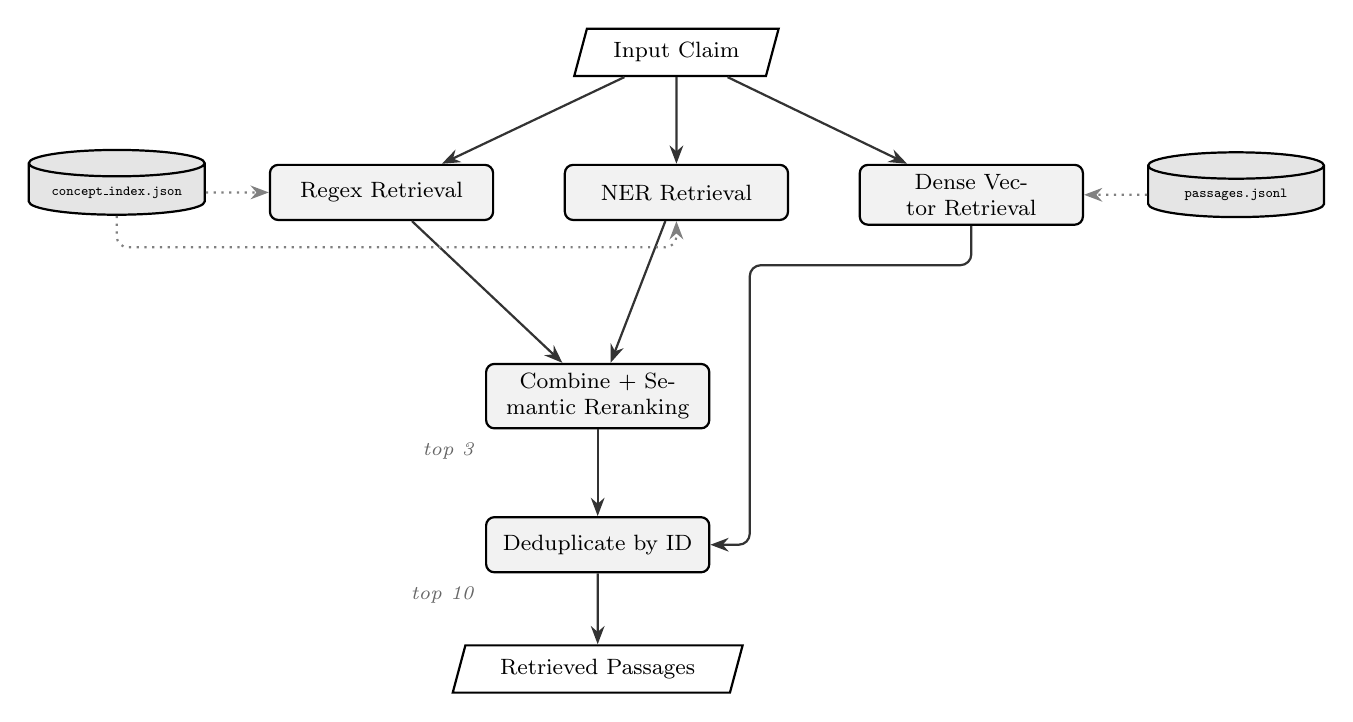
\begin{tikzpicture}[node distance=0.9cm and 0.5cm]
  % Input
  \node[io] (claim) {Input Claim};

  % Three parallel retrievers — evenly spaced row
  \node[process, below left=1.1cm and 2.0cm of claim] (regex)
    {Regex Retrieval};
  \node[process, below=1.1cm of claim] (ner)
    {NER Retrieval};
  \node[process, below right=1.1cm and 2.0cm of claim] (dense)
    {Dense Vector Retrieval};

  % Combine — centered below regex and ner
  \node[process, below=1.8cm of ner, xshift=-1.0cm] (combine)
    {Combine + Semantic Reranking};

  % Deduplicate — below combine
  \node[process, below=1.1cm of combine] (dedup)
    {Deduplicate by ID};

  % Output
  \node[io, below=0.9cm of dedup] (out)
    {Retrieved Passages};

  % Data stores — beside their retrievers
  \node[datastore, left=0.8cm of regex] (cidx)
    {\texttt{concept\_index.json}};
  \node[datastore, right=0.8cm of dense] (pass)
    {\texttt{passages.jsonl}};

  % Arrows from claim to retrievers
  \draw[arrow] (claim) -- (regex);
  \draw[arrow] (claim) -- (ner);
  \draw[arrow] (claim) -- (dense);

  % Regex and NER to combine
  \draw[arrow] (regex) -- (combine);
  \draw[arrow] (ner) -- (combine);

  % Combine to dedup
  \draw[arrow] (combine) -- (dedup);

  % Dense vector bypass — route along right edge to dedup
  \draw[arrow, rounded corners=4pt] (dense.south) -- ++(0,-0.5) -| ([xshift=0.5cm]dedup.east) -- (dedup.east);

  % Dedup to output
  \draw[arrow] (dedup) -- (out);

  % Data store dependencies
  \draw[-Stealth, dotted, thick, black!50] (cidx) -- (regex);
  \draw[-Stealth, dotted, thick, black!50, rounded corners=4pt]
    (cidx.south) -- ++(0,-0.4) -| (ner.south);
  \draw[-Stealth, dotted, thick, black!50] (pass) -- (dense);

  % Annotations
  \node[annot, below left=0.05cm and 0.02cm of combine] {top 3};
  \node[annot, below left=0.05cm and 0.02cm of dedup] {top 10};
\end{tikzpicture}
}
\caption{Subgrafo de recuperación híbrida. Tres rutas paralelas---regex, NER y vectores densos---se fusionan y deduplican para producir el conjunto final de evidencia.}
\label{fig:retrieval}
\end{figure*}


\end{document}
